\documentclass{standalone} % Utilise la classe standalone pour compiler uniquement le TikZ
\usepackage{tikz}          % Charge le package TikZ
\usepackage{xcolor}        % Gestion avancée des couleurs
\usepackage{amsmath}       % Gestion des formules mathématiques
\usetikzlibrary{arrows.meta} % Pour gérer les flèches avec des formes spécifiées comme "triangle"
\usetikzlibrary {decorations.pathmorphing}
\usepackage{pgfplots}
%\pgfplotsset{compat=1.18}
%\usepgfplotslibrary{external}
%\tikzexternalize


% Définition de la fonction pour générer la grille
\newcommand{\drawgrid}[4]{


	\begin{scope}[opacity = 0.2]
	
	
    	% Paramètres : #1=xmin, #2=xmax, #3=ymin, #4=ymax

   	 	% Grille principale en cm
    	\draw[very thin, gray] (#1,#3) grid (#2,#4); % Grille de base (1 cm)
    
    	\draw[very thin, gray] (#1,#3) grid[step=0.1] (#2,#4);

    	\draw[thin, black] (#1,#3) edge[thick,line width=0.8ex,->,>=Stealth ] (#2,#3); 
    
    	\foreach \x in {#1,..., #2} {
        	\draw[shift={(\x, #3)}] (0,-0.1) edge[line width=0.8ex] node[pos = -1 , below] {\x} (0,0.1); % Lignes verticales en mm
    	}

    	\draw[thin, black] (#1,#3)edge[thick,line width=0.8ex,->,>=Stealth ] (#1,#4); 
    
    	\foreach \y in {#3,..., #4} {
        	\draw[shift={(#1, \y)}] (-0.1 , 0 ) edge[line width=0.8ex] node[pos = -1 , left ] {\y} (0.1 , 0); % Lignes verticales en mm
    	}
    
    \end{scope}


}


\newcommand{\Axex}[1][$x$]{ % "x" est la valeur par défaut de #1
    \draw
        (-10, 0) edge[thick, line width=0.8ex, ->, >=Triangle, color=\colorThree] 
        node[shift = {(0,1)} , pos=1.01, below]{ \huge #1 } (10, 0)
        ;
}

\newcommand{\Axetheta}[1][$\theta$]{
	\draw
		(-10, 0 ) edge [thick,line width=0.8ex,->,>=Triangle , color = \colorThree ]node [pos=1.01,right]{\huge #1 } ( 10  , 0 )
	;
}

\newcommand{\Axedensity}[1][$n$]{
	\draw
		(0, -1 ) edge [thick,line width=0.8ex,->,>=Triangle , color = \colorThree ]node [pos=1.01,left  ]{\huge #1 } ( 0  , 6 )
	;
}

\newcommand{\Axedistribution}[1][$\nu$]{
	\draw
		(0, -1 ) edge [thick,line width=0.8ex,->,>=Triangle , color = \colorThree ]node [pos=1.01,left  ]{\huge #1 } ( 0  , 6 )
	;
}

\newcommand{\Axesphase}[2][$x$]{
	\Axex[#1]
	\begin{scope}[rotate = 90]
		\Axetheta[#2]	
	\end{scope}
}

\newcommand{\Axesdensity}[2][$x$]{
	\Axex[#1]
	\Axedensity[#2]
}

\newcommand{\Axesdistribution}[2][\theta]{
	\Axetheta[#1]
	\Axedistribution[#2]
}

\newcommand{\Axetemps}[1][Deformation]{
	\draw 
		(-5 , 0 ) edge [line width=2.8ex, color=\colorOne ]( 0, 0)
		(43 , 0 ) edge [line width=2.8ex, color=\colorOne , ->, >=Triangle] node[pos = 1.0 , right , scale = 2 ] { \fontsize{60pt}{720pt}\selectfont $\tilde{t}$} ( 50 , 0)
		( 0 , 1 ) edge [line width=2.0ex, color=\colorOne ] ( 0 , -1 )  
		( 43 , 1 ) edge [line width=2.0ex, color=\colorOne ] ( 43 , -1 ) 
		(0 , 0) edge[<->, > = stealth, line width=2.8ex, color=\colorOne ]  node [ rectangle , midway, fill = white , scale = 2 ] {\fontsize{600pt}{720pt}\selectfont \bf  #1}(43, 0)  
	;

}

\newcommand{\Palette}[1][\colorOne]{
	\clip[decorate, decoration={random steps, segment length=3pt, amplitude=3pt}]
        	(-1,-1) rectangle (1,1);
	\draw[fill=#1 , color = #1 ] (-2,-2) rectangle (2,2);
}


\begin{document}



% Définition des couleurs avec les codes HTML
\definecolor{colorOne}{HTML}{443E46}
\definecolor{colorTwo}{HTML}{F6DEB8}
\definecolor{colorThree}{HTML}{908CA4}
\definecolor{colorFour}{HTML}{57659E}
\definecolor{colorFive}{HTML}{C57284}
\definecolor{colorSix}{HTML}{FF5B69}

% Raccourcis pour les couleurs
\def\colorOne{colorOne}
\def\colorTwo{colorTwo}
\def\colorThree{colorThree}
\def\colorFour{colorFour}
\def\colorFive{colorFive}
\def\colorSix{colorSix}




\def\Background{
	\draw[fill = \colorFour ]  
		(-10 , -10 ) rectangle ( 10 , 10 ) 
	;	

}





%% different test d'insitut 

% a la main
\pgfdeclareverticalshading{Insitut}{20cm}
 {color(0)=(\colorFour); color(2cm)=(\colorFive); color(4cm)=(\colorSix);color(10cm)=(\colorSix);  color(12cm)=(\colorFive);  color(14cm)=(\colorFour)}
 % avec donné
\newcommand{\Insitutmap}[0]{
 \begin{axis}[
	%title={Données expérimentales $f(x,y)$},
    colormap/viridis,
    %colorbar,
    enlargelimits=false,
    axis on top,
    xtick=\empty,
    ytick=\empty,
    xlabel={},
    ylabel={},
    axis lines=none
]

\addplot [
    matrix plot,
    point meta=explicit,
    mesh/rows=5, % à adapter au nombre de lignes
    shader=interp,
]
table [meta=z] {./data/donnees1.dat};
\end{axis}
}



\begin{tikzpicture}

% Placement de l'axe défini dans un cercle avec une échelle globale
%\Axes 

%% Pour voir plus precisement 
\clip (-21 , -85) rectangle (58 , 21) ;\draw[color = red ] (-20 , -84) rectangle (58 , 20) ;
%\clip (-20 , -15) rectangle (20 , 20) ; \draw[color = red ] (-20 , -14) rectangle (20 , 18) ; % voire Insitut
%\clip (10 , -15) rectangle (55 , 20) ; \draw[color = red ] (10 , -15) rectangle (55 , 20) ; % voire coupure 1 0ms  
%\clip (53 , -15) rectangle (95 , 20) ; \draw[color = red ] (53 , -15) rectangle (95 , 20) ; % voire coupure 1 18ms 
%\clip (53 , -55) rectangle (95 , 20) ; \draw[color = red ] (53 , -55) rectangle (95 , 20) ; % voire coupure 1 18ms 



% palette de couleur 
\node at (40,6) [rectangle , rotate = -90] { 
	\begin{tikzpicture}
	
	\node at (0,0) [rectangle, ] {
		\begin{tikzpicture}
			\Palette[\colorOne]
		\end{tikzpicture}} ;
	\node at (3,0) [rectangle, ] {
		\begin{tikzpicture}
			\Palette[\colorTwo]
		\end{tikzpicture}} ;
	\node at (6,0) [rectangle, ] {
		\begin{tikzpicture}
			\Palette[\colorThree]
		\end{tikzpicture}} ;
	\node at (9,0) [rectangle, ] {
		\begin{tikzpicture}
			\Palette[\colorFour]
		\end{tikzpicture}} ;
	\node at (12,0) [rectangle, ] {
		\begin{tikzpicture}
			\Palette[\colorFive]
		\end{tikzpicture}} ;
	\node at (15,0) [rectangle, ] {
		\begin{tikzpicture}
			\Palette[\colorSix]
		\end{tikzpicture}} ;
	
	\end{tikzpicture}
	}; 
	

% Insitut 	
\node at (21,0) [rectangle ]{
	\begin{tikzpicture}[transform canvas={scale=1}] 
		
		% diagrale de phase 
		\node at (0,0) [circle, ] {
			\begin{tikzpicture}[transform canvas={scale=1}] 
				
				%\node at (0,0) [circle, ]{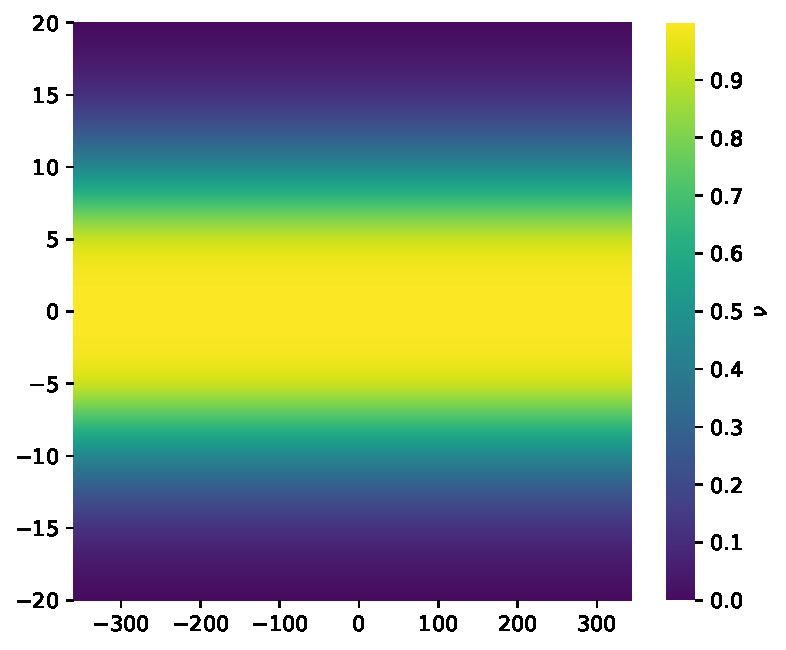
\includegraphics[width=2\textwidth]{data/insitut.pdf}};

				\begin{scope}
	 				% Appliquer un rectangle décoré et clipper la zone
    				%\clip[decorate, decoration={random steps, segment length=3pt, amplitude=1pt}](-8,-8) rectangle (8,8); 
     				%\node at (0,0) [circle  ] {\begin{tikzpicture}[transform canvas={scale=1}] \Background \end{tikzpicture}};
					%\node at (0,0) [circle, ] {\pgfuseshading{Insitut}};
					%\node at (0,0) [circle, ] {\begin{tikzpicture} \Insitutmap \end{tikzpicture} };
					\node at (-0.95,-0.3) [circle, ]{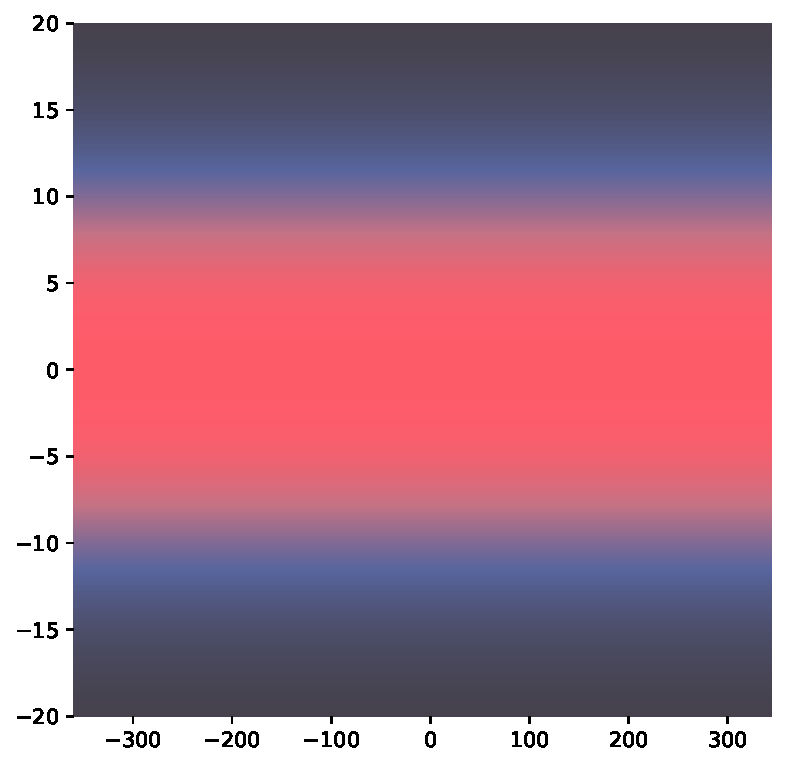
\includegraphics[height = 1.6\textwidth]{data/graph_insitut_only.pdf}}; %width=1.8\textwidth
					%\node at (0,0) [circle, ]{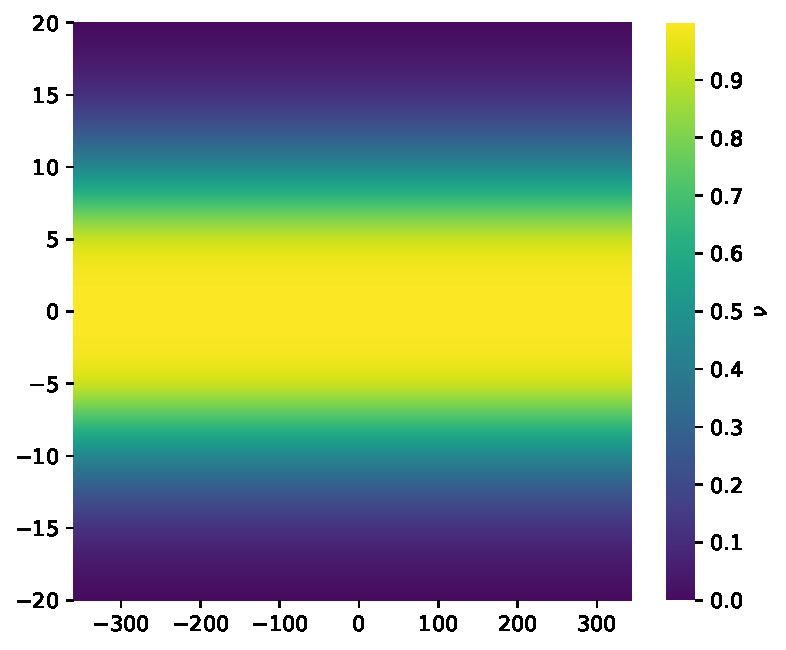
\includegraphics[height = 1.6\textwidth]{data/insitut.pdf}}; 
		
				\end{scope}
				
				\begin{scope}[shift={(2,-0.3)}]
					\clip[decorate, decoration={random steps, segment length=3pt, amplitude=1pt}](9,-9) rectangle (13,10);
					%\draw[red]  (9,-9) rectangle (13,10);	
					\node at (0,0) [circle, ]{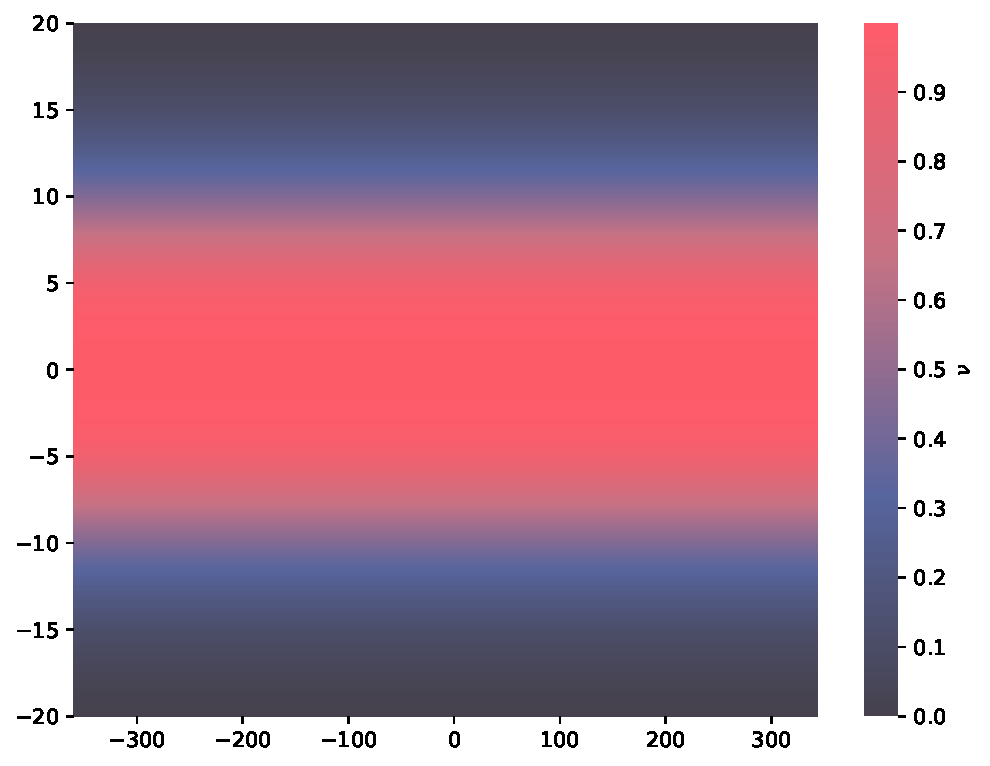
\includegraphics[height = 1.6\textwidth ]{data/complete_graph_insitut.pdf}}; 
				\end{scope}

				%\node at (0,0) [circle, ]{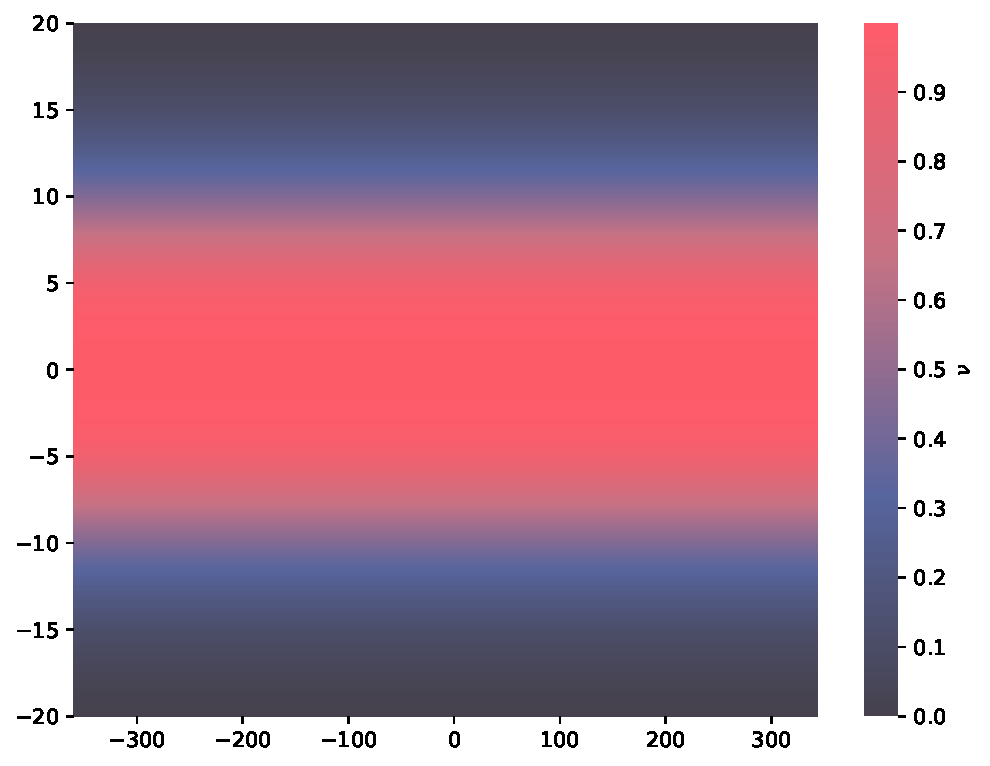
\includegraphics[width = 1.8\textwidth , trim=0cm 0.cm 0cm 0.cm, clip ]{data/complete_graph_insitut.pdf}}; 
				
				\node at (0,0) [circle] { \begin{tikzpicture}[transform canvas={scale=1}] \Axesphase[$x ~ (\mu m) $]{$\theta ~ (\mu m / {ms}) $} \end{tikzpicture}};

			\end{tikzpicture}
			};
	
		% density 
		\node at (0,13) [circle, ] {
			\begin{tikzpicture}[transform canvas={scale=1}] 
				\begin{scope}
					\clip[decorate, decoration={random steps, segment length=3pt, amplitude=1pt}]
        			(-9,-8) rectangle (8.5,8); 
        			\draw[line width=1.8ex , color = \colorFour , fill = none ] (-10 , 0 ) -- (-10 , 5 ) -- (10 , 5 ) -- ( 10, 0 )  ;
        			\draw[line width=1.8ex , color = \colorFour] 
        				(-0.3, 5 ) edge [thick,line width=0.8ex,, color = \colorThree ]node [pos=-0.01, left  ]{\huge $56$ } ( 0.3  , 5 )	
        				(-0.3, 0 ) edge [thick,line width=0.8ex,, color = \colorThree ]node [pos=-0.01, below left ]{\huge $0$ } ( 0.3  , 0 )	
        			;	
								
				\end{scope}
		
				\Axesdensity[$x ~ (\mu m) $]{$n ~({\mu m}^{-1})$}
		
			\end{tikzpicture}

			};
	
	
		% distribution
		\node at (-13,0) [circle, rotate = 90 ] {
			\begin{tikzpicture}[transform canvas={scale=1}] 
				\begin{scope}
					\clip[decorate, decoration={random steps, segment length=3pt, amplitude=1pt}](-8.8,-8) rectangle (8.8,8);

					%\filldraw[smooth , line width=1.8ex , color = \colorFour , fill = \colorThree] plot coordinates {(-10,0) (-5,0.5) (-4,4) (4,4) (5,0.5) (10 , 0 )};
					%\filldraw[  smooth, line width=1.8ex, color=\colorFour, fill=\colorThree] (-10,0)  .. controls (0,0) and (-10,5) .. (0,5) .. controls (10,5) and (0,0) .. (10,0);	
    				\draw[line width=1.8ex , color = \colorFour , fill = none ] plot[smooth] file {data/insitut.table};
    				\draw[line width=1.8ex , color = \colorFour] 
    					(-0.3, 5 ) edge [thick,line width=0.8ex, color = \colorThree ]node [pos=-0.01, left  ]{\huge $1$ } ( 0.3  , 5 )	
    					(-0.3, 0 ) edge [thick,line width=0.8ex,, color = \colorThree ]node [pos=-0.01, below left ]{\huge $0$ } ( 0.3  , 0 )	
    					;	
    						
				\end{scope}		
				\Axesdistribution[$\theta ~ (\mu m / {ms}) $]{$\nu$}	
			\end{tikzpicture}

			};

	\end{tikzpicture}
};

% coupuur 1 O ms	
\node at (0,-35) [rectangle ]{
	\begin{tikzpicture}[transform canvas={scale=1}] 
		
		% diagrale de phase 
		\node at (0,0) [circle, ] {
			\begin{tikzpicture}[transform canvas={scale=1}] 
				\begin{scope}
	 				% Appliquer un rectangle décoré et clipper la zone
    				%\clip[decorate, decoration={random steps, segment length=3pt, amplitude=1pt}](-8,-8) rectangle (8,8); 
     				%\node at (0,0) [circle  ] {\begin{tikzpicture}[transform canvas={scale=1}] \Background \end{tikzpicture}};
     				%\clip (0,-8) rectangle (10,8) ;
					%\node at (0,0) [circle, ] {\pgfuseshading{Insitut}};
					\node at (-0.95,-0.3) [circle, ]{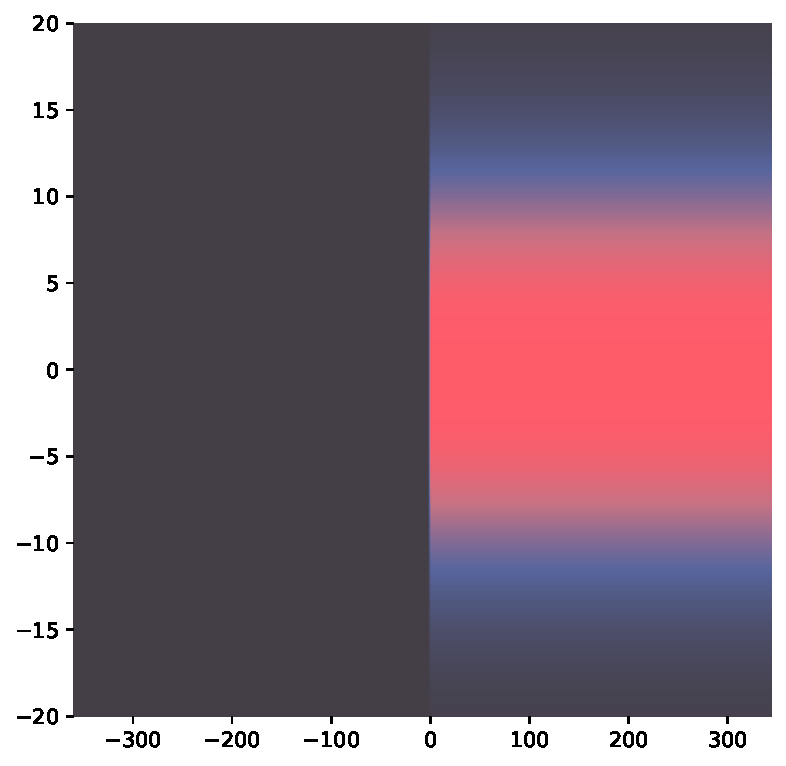
\includegraphics[height = 1.6\textwidth]{data/graph_coupure_1_0_only.pdf}};
		
				\end{scope}
				
				\draw[opacity = 0.5 , dashed , line width=1.8ex , color = \colorTwo , fill = none] 
					plot[smooth] file {data/bord_0_0.table}
					(-7,7) edge []node [pos=1.1, right ]{\huge $bord$ } ( -6.5  , 7 )	 
				;
				
				\node at (0,0) [circle, ] {\begin{tikzpicture}[transform canvas={scale=1}] \Axesphase[$x ~ (\mu m)$]{$\theta ~ (\mu m / {ms}) $} \end{tikzpicture}};

			\end{tikzpicture}
			};
	
		% density 
		\node at (0,13) [circle, ] {
			\begin{tikzpicture}[transform canvas={scale=1}] 
				\begin{scope}
					\clip[decorate, decoration={random steps, segment length=3pt, amplitude=1pt}](-9,-8) rectangle (8.5,8);
 					
        			\filldraw[line width=1.8ex , color = \colorFour , fill = none ] 
						(-10 , 0 ) --  ( 0 , 0 ) -- ( 0 , 5 ) --(10 , 5 ) -- ( 10 , 0 )   
					;
					\draw[opacity = 1 , line width=1.8ex , dashed , color = \colorThree , fill = none ] (-10 , 0 ) -- (-10 , 5 ) -- (10 , 5 ) -- ( 10, 0 )  ;
					
					\draw[line width=1.8ex , color = \colorFour] 
        				(-0.3, 5 ) edge [thick,line width=0.8ex,, color = \colorThree ]node [pos=-0.01, left  ]{\huge $56$ } ( 0.3  , 5 )	
        				(-0.3, 0 ) edge [thick,line width=0.8ex,, color = \colorThree ]node [pos=-0.01, below left ]{\huge $0$ } ( 0.3  , 0 )	
        			;				
				\end{scope}
				
				\draw 
					(-8,4) edge [thick,line width=1.8ex,opacity = 0.3 , dashed , color = \colorFour ]node [pos=1.1, right ]{\huge $n( t = 0^{-})$ } ( -7.5  , 4 )	
    				(-8,3) edge [thick,line width=1.8ex , color = \colorFour ]node [pos=1.1, right ]{\huge $n( t = 0^{+} )$ } ( -7.5  , 3 )	
    				
    			;
		
				\Axesdensity[$x ~ (\mu m) $]{$n ~({\mu m}^{-1})$}
				%\drawgrid{-10}{10}{-10}{10}
			\end{tikzpicture}

			};
		
		% distribution x < 0 
		\node at (-13,0) [circle,   rotate = 90 , xscale = 1   ] {
			\begin{tikzpicture}[transform canvas={scale=1} ] 
				\begin{scope}
					\clip[decorate, decoration={random steps, segment length=3pt, amplitude=1pt}](-8.8,-8) rectangle (8.8,8);

					%\filldraw[smooth , line width=1.8ex , color = \colorFour , fill = \colorThree] plot coordinates {(-10,0) (-5,0.5) (-4,4) (4,4) (5,0.5) (10 , 0 )};
					%\filldraw[  smooth, line width=1.8ex, color=\colorFour, fill=\colorThree] (-10,0)  .. controls (0,0) and (-10,5) .. (0,5) .. controls (10,5) and (0,0) .. (10,0);	
					

    				\filldraw[smooth , line width=1.8ex , color = \colorFour , fill = none] plot coordinates {(-10,0)  (10 , 0 )};
    				\draw[opacity = 0.3 , dashed , line width=1.8ex , color = \colorFour , fill = none] plot[smooth] file {data/insitut.table};
    				
    				\draw[line width=1.8ex , color = \colorFour]     	
    					(-0.3, 5 ) edge [thick,line width=0.8ex, color = \colorThree ]node [pos=-0.01, left  ]{\huge $1$ } ( 0.3  , 5 )	
    					(-0.3, 0 ) edge [thick,line width=0.8ex,, color = \colorThree ]node [pos=-0.01, below left ]{\huge $0$ } ( 0.3  , 0 )	
    					;				
				\end{scope}	
				
				\draw 
					(4,5) edge [thick,line width=1.8ex,opacity = 0.3 , dashed , color = \colorFour ]node [pos=1.1, right ]{\huge $\nu(x < 0 ; t = 0^{-})$ } ( 4.5  , 5 )	
    				(4,4) edge [thick,line width=1.8ex , color = \colorFour ]node [pos=1.1, right ]{\huge $\nu(x < 0 ; t = 0^{+} )$ } ( 4.5  , 4 )	
    				
    			;	
				\Axesdistribution[$\theta ~ (\mu m / {ms}) $]{$\nu ( x < 0 ) $}	
			\end{tikzpicture}

			};
	
		% distribution x > 0 
		\node at (13,0) [circle,   rotate = 90 , yscale = 1   ] {
			\begin{tikzpicture}[transform canvas={scale=1} ] 
				\begin{scope}
					\clip[decorate, decoration={random steps, segment length=3pt, amplitude=1pt}](-8.8,-8) rectangle (8.8,8);

					%\filldraw[smooth , line width=1.8ex , color = \colorFour , fill = \colorThree] plot coordinates {(-10,0) (-5,0.5) (-4,4) (4,4) (5,0.5) (10 , 0 )};
					%\filldraw[  smooth, line width=1.8ex, color=\colorFour, fill=\colorThree] (-10,0)  .. controls (0,0) and (-10,5) .. (0,5) .. controls (10,5) and (0,0) .. (10,0);	
    				\draw[line width=1.8ex , color = \colorFour , fill = none] plot[smooth] file {data/insitut_minus.table};
    				\draw[line width=1.8ex , color = \colorFour] 
    					(-0.3, -5 ) edge [thick,line width=0.8ex, color = \colorThree ]node [pos=-0.01, left  ]{\huge $1$ } ( 0.3  , -5 )	
    					(-0.3, 0 ) edge [thick,line width=0.8ex,, color = \colorThree ]node [pos=-0.01, above left ]{\huge $0$ } ( 0.3  , 0 )	
    					;			
				\end{scope}	
				
				\draw
					(-10, 0 ) edge [thick,line width=0.8ex,->,>=Triangle , color = \colorThree ]node [pos=1.01,right]{\huge $\theta ~ (\mu m / {ms}) $ } ( 10  , 0 )
					(0, 1 ) edge [thick,line width=0.8ex,->,>=Triangle , color = \colorThree ]node [pos=1.01,left  ]{\huge $\nu ( x > 0 ) $ } ( 0  , -6 )
				;	
				%\Axesdistribution[$\theta ~ (\mu m / {ms}) $]{$\nu ( x > 0 ) $}		
			\end{tikzpicture}

			};

	\end{tikzpicture}
};


% coupuur 1 18 ms	
\node at (43,-35) [rectangle ]{
	\begin{tikzpicture}[transform canvas={scale=1}] 
		
		% diagrale de phase 
		\node at (0,0) [circle, ] {
			\begin{tikzpicture}[transform canvas={scale=1}] 
				\begin{scope}
	 				% Appliquer un rectangle décoré et clipper la zone
    				%\clip[decorate, decoration={random steps, segment length=3pt, amplitude=1pt}](-8,-8) rectangle (8,8); 
     				%\node at (0,0) [circle  ] {\begin{tikzpicture}[transform canvas={scale=1}] \Background \end{tikzpicture}};
     				%\clip[smooth] plot coordinates {(-5,-10) (-2,-2.75) (2,2.75) (5,10) (10,10) (10 , -10 )} ;
					%\node at (0,0) [circle, ] {\pgfuseshading{Insitut}};
					\node at (-0.95,-0.3) [circle, ]{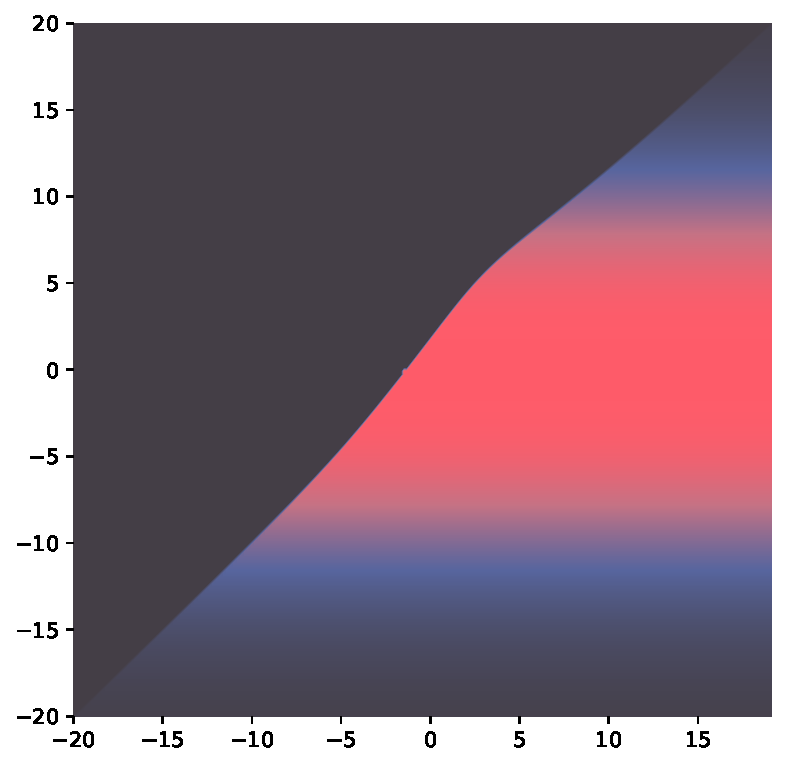
\includegraphics[height = 1.6\textwidth]{data/graph_coupure_1_18_only.pdf}};
		
				\end{scope}
				\begin{scope}[shift={(2,-0.3)}]
					\clip[decorate, decoration={random steps, segment length=3pt, amplitude=1pt}](9,-9) rectangle (13,10);
					%\draw[red]  (9,-9) rectangle (13,10);	
					\node at (0,0) [circle, ]{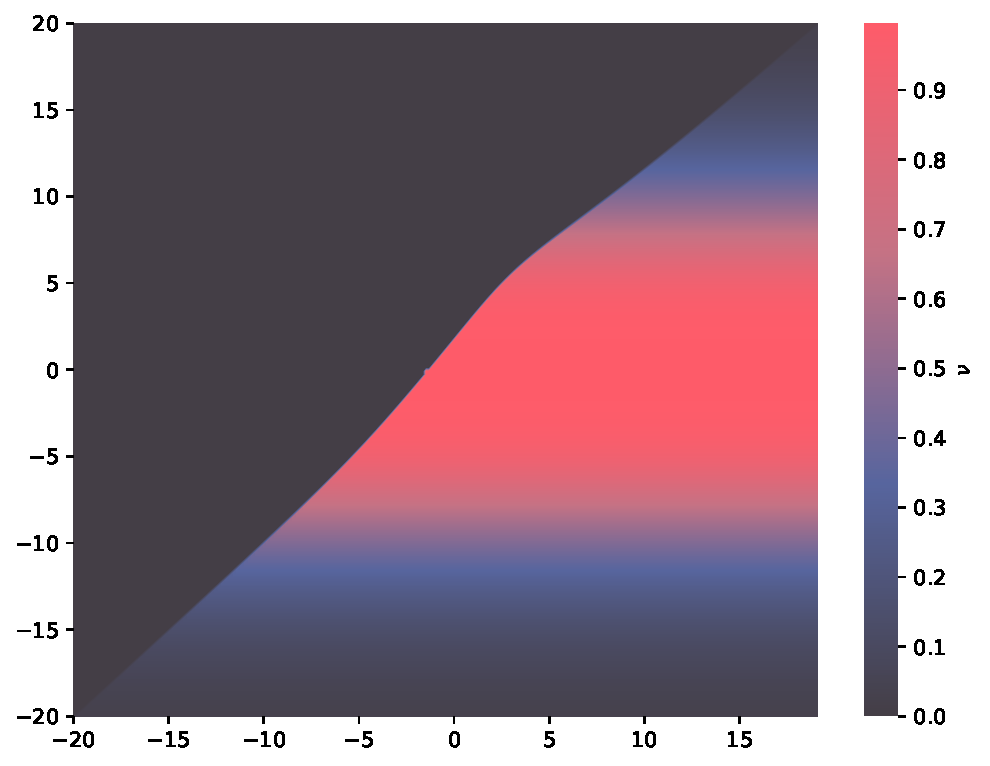
\includegraphics[height = 1.6\textwidth ]{data/complete_graph_coupure_1_18.pdf}}; 
				\end{scope}
				\node at (0,0) [circle, ] {
					\begin{tikzpicture}[transform canvas={scale=1}] 
						\Axesphase[$x/t ~ (\mu m / ms) $]{$\theta ~ (\mu m / {ms}) $}
						\draw
    						(1, 0.2) edge[line width=1.8ex, color=\colorTwo] 
        						node[pos=1.1, below]{ \color{\colorTwo}\huge $x(s)/t$} (1, -0.2)
        					(0.2 , 2 ) edge[line width=1.8ex, color=\colorTwo] 
        						node[pos=1.1, left ]{ \color{\colorTwo}\huge $\theta(s)$} (-0.2 , 2 )
        					(1 , -0.2 ) edge[line width=0.8ex, color=\colorTwo , dashed ] (1 , 2.5 )
        					(-0.2 , 2 )  edge[line width=0.8ex, color=\colorTwo , dashed ] (1.5  , 2 )
        					;
        					
					\end{tikzpicture}};
				\draw[opacity = 0.5 , dashed , line width=1.8ex , color = \colorTwo , fill = none] 
					plot[smooth] file {data/bord_0_sur_18.table}
					(-7,7) edge []node [pos=1.1, right ]{\huge $bord : v^{\mbox{\tiny eff}}$ } ( -6.5  , 7 )	 
				;
				%\drawgrid{-10}{10}{-10}{10}
			\end{tikzpicture}
			};
	
		% density 
		\node at (0,13) [circle, ] {
			\begin{tikzpicture}[transform canvas={scale=1}] 
				\begin{scope}
					\clip[decorate, decoration={random steps, segment length=3pt, amplitude=1pt}](-9,-8) rectangle (8.3,8);
 
        			%\filldraw[smooth , line width=1.8ex , color = \colorFour , fill = \colorThree ] plot coordinates {(-10,0) (-3,0.4) (2.,4.5) (10,5) 
     				 %(10 , 0 )};
     				 %\filldraw[smooth, line width=1.8ex, color=\colorFour, fill=\colorThree] (-10,0) -- (-2,0) .. controls (-1,0) and (2,5) .. (3,5) -- (10,5) -- (10,0);
     				 \draw[opacity = 1 , line width=1.8ex , color = \colorFour , fill = none ] plot[] file {data/density_coupure_1_sur_18.table};
     				 \draw[line width=1.8ex , color = \colorFour] 
        				(-0.3, 5 ) edge [thick,line width=0.8ex,, color = \colorThree ]node [pos=-0.01, left  ]{\huge $56$ } ( 0.3  , 5 )	
        				(-0.3, 0 ) edge [thick,line width=0.8ex,, color = \colorThree ]node [pos=-0.01, below left ]{\huge $0$ } ( 0.3  , 0 )	
        			;	


				\end{scope}
		
				\Axesdensity[$x/t ~ (\mu m / ms)$]{$n ~ ({\mu m}^{-1})$}
				

        				
				%\drawgrid{-10}{10}{-10}{10}
		
			\end{tikzpicture}

			};
		
		% distribution x  
		\node at (-13,0) [circle,   rotate = 90 , xscale = 1   ] {
			\begin{tikzpicture}[transform canvas={scale=1} ] 
				\begin{scope}
					\clip[decorate, decoration={random steps, segment length=3pt, amplitude=1pt}](-8.8,-8) rectangle (8.8,8);

					%\filldraw[smooth , line width=1.8ex , color = \colorFour , fill = \colorThree] plot coordinates {(-10,0) (-5,0.5) (-4,4) (4,4) (5,0.5) (10 , 0 )};
					
					%\filldraw[ opacity = 0.5 , smooth, line width=1.8ex, color=\colorFour, fill=\colorThree] (-10,0)  .. controls (0,0) and (-10,5) .. (0,5) .. controls (10,5) and (0,0) .. (10,0);
    				
					
					%\filldraw[  opacity = 1 , smooth, line width=1.8ex, color=\colorFour, fill=\colorThree] (-10,0)  .. controls (0,0) and (-10,5) .. (0,5) .. controls (1.3,5) and (1.3,5) .. (1.3,4.9) -- (1.3 , 0 )-- ( 10 , 0 ) ;
    						
    				\draw[opacity = 1 , line width=1.8ex , color = \colorFour , fill = none ] plot[] file {data/coupure_1_sur_18.table};	
    				
    				\draw[opacity = 0.3 , line width=1.8ex , dashed ,  color = \colorFour , fill = none] plot[smooth] file {data/insitut.table};
    				
    				\draw[line width=1.8ex , color = \colorFour] 
    					(-0.3, 5 ) edge [thick,line width=0.8ex, color = \colorThree ]node [pos=-0.01, left  ]{\huge $1$ } ( 0.3  , 5 )	
    					(-0.3, 0 ) edge [thick,line width=0.8ex,, color = \colorThree ]node [pos=-0.01, below left ]{\huge $0$ } ( 0.3  , 0 )		
    					;			
				\end{scope}
				\draw
    				(2, 0.2) edge[line width=1.8ex, color=\colorOne] 
        				node[pos=1.1, below]{ \color{\colorThree}\huge $\theta(s)$} (2, -0.2)
        				
        			(4,5) edge [thick,line width=1.8ex,opacity = 0.3 , dashed , color = \colorFour ]node [pos=1.1, right ]{\huge $\nu(x(s); t = 0^{-})$ } ( 4.5  , 5 )	
    				(4,4) edge [thick,line width=1.8ex , color = \colorFour ]node [pos=1.1, right ]{\huge $\nu(x(s); t = 18 ~ms )$ } ( 4.5  , 4 )	
        		;		
				\Axesdistribution[$\theta ~ (\mu m/ms)$]{$\nu ( x(s) ) $}
				
				%\drawgrid{0}{10}{-10}{10}	
			\end{tikzpicture}

			};
	

	\end{tikzpicture}
};

%axe temporel 
\node at (0, -47) [circle ]{
	\begin{tikzpicture}[transform canvas={scale=1} ]
		\Axetemps[Déformation : $t = 18 ~ms$]
	\end{tikzpicture}
	};




% coupuur 2 0 ms	
\node at (0,-70) [rectangle ]{
	\begin{tikzpicture}[transform canvas={scale=1}] 
		
		% diagrale de phase 
		\node at (0,0) [circle, ] {
			\begin{tikzpicture}[transform canvas={scale=1}] 
				\begin{scope}
	 				% Appliquer un rectangle décoré et clipper la zone
    				%\clip[decorate, decoration={random steps, segment length=3pt, amplitude=1pt}](-8,-8) rectangle (8,8); 
     				%\node at (0,0) [circle  ] {\begin{tikzpicture}[transform canvas={scale=1}] \Background \end{tikzpicture}};
     				%\clip[smooth] plot coordinates {(-5,-10) (-2,-2.75) (2,2.75) (5,10) (10,10)  (10 , -10 )} ;
     				 %\clip (0.75,-10) rectangle (1.25 , 10 ) ;
					%\node at (0,0) [circle, ] {\pgfuseshading{Insitut}};
					\node at (-0.95,-0.3) [circle, ]{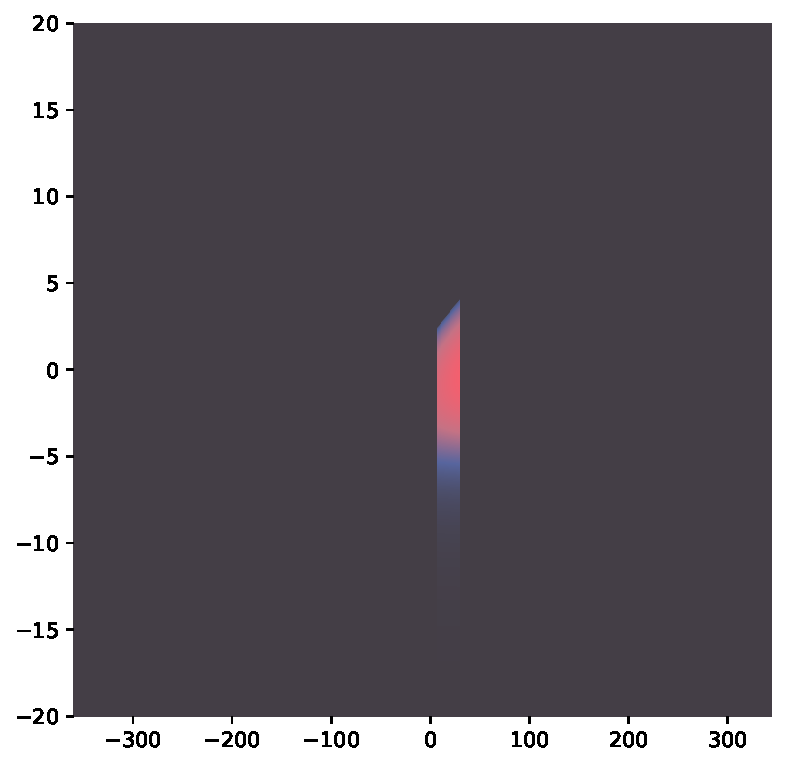
\includegraphics[height = 1.6\textwidth]{data/graph_coupure_2_0_only.pdf}};
		
				\end{scope}
				\begin{scope}[shift={(2,-0.3)}]
					\clip[decorate, decoration={random steps, segment length=3pt, amplitude=1pt}](8.5,-9) rectangle (13,10);
					%\draw[red]  (9,-9) rectangle (13,10);	
					\node at (0,0) [circle, ]{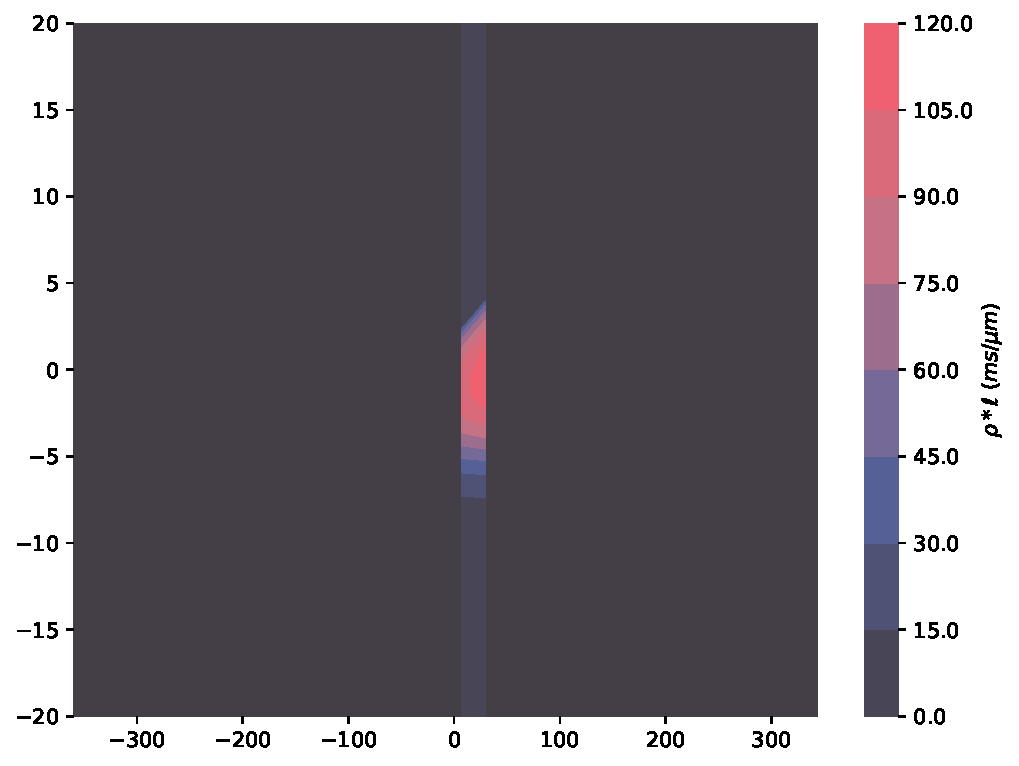
\includegraphics[height = 1.6\textwidth ]{data/complete_graph_coupure_2_0.pdf}}; 
				\end{scope}
				\node at (0,0) [circle, ] {
					\begin{tikzpicture}[transform canvas={scale=1}] 
						\Axesphase[$x~(\mu m)$]{$\theta~(\mu m/ms)$}
						\draw
    						(0.45, 0.2) edge[line width=1.8ex, color=\colorTwo] 
        						node[pos=1.1, below]{ \color{\colorTwo}\huge $x(s)$} (0.45, -0.2)
        					(0.2 , 1.4 ) edge[line width=1.8ex, color=\colorTwo] 
        						node[pos=1.1, left ]{ \color{\colorTwo}\huge $\theta(s)$} (-0.2 , 1.4 )
        					(0.45 , -0.2 ) edge[line width=0.8ex, color=\colorTwo , dashed ] (0.45 , 2 )
        					(-0.2 , 1.4 )  edge[line width=0.8ex, color=\colorTwo , dashed ] (1.0  , 1.4 )
        					; 
					\end{tikzpicture}};
					\draw[opacity = 0.3 , dashed , line width=0.5ex , color = \colorTwo , fill = none] 
						plot[smooth] file {data/bord_0_sur_18.table}
						(-7,7) edge []node [pos=1.1, right ]{\huge $bord~v^{\mbox{\tiny{eff}}}$ } ( -6.5  , 7 )	 
					;
					\draw[opacity = 0.5 , dotted , line width=0.5ex , color = \colorTwo , fill = none] 
						plot[smooth] file {data/bord_1_0.table}
						(-7,6) edge []node [pos=1.1, right ]{\huge $bord~gauche$ } ( -6.5  , 6 )	 
					;
					\draw[opacity = 0.5 , dash dot , line width=0.5ex , color = \colorTwo , fill = none] 
						plot[smooth] file {data/bord_2_0.table}
						(-7,5) edge []node [pos=1.1, right ]{\huge $bord~droite$ } ( -6.5  , 5 )	 
					;
				%\drawgrid{-10}{10}{-10}{10}
			\end{tikzpicture}
			};
	
		% density 
		\node at (0,13) [circle, ] {
			\begin{tikzpicture}[transform canvas={scale=1}] 
				\begin{scope}
					\clip[decorate, decoration={random steps, segment length=3pt, amplitude=1pt}]
        			(-9,-8) rectangle (8.3,8);
 
        			\draw[opacity = 0.3 , line width=1.8ex , dashed ,  color = \colorFour , fill = none ] plot[] file {data/density_coupure_1_sur_18.table};
        			\draw[opacity = 1 , line width=1.8ex , color = \colorFour , fill = none ] plot[] file {data/density_coupure_2_0.table};
     				 \draw[line width=1.8ex , color = \colorFour] 
        				(-0.3, 5 ) edge [thick,line width=0.8ex,, color = \colorThree ]node [pos=-0.01, left  ]{\huge $56$ } ( 0.3  , 5 )	
        				(-0.3, 0 ) edge [thick,line width=0.8ex,, color = \colorThree ]node [pos=-0.01, below left ]{\huge $0$ } ( 0.3  , 0 )	
        			;

					%\drawgrid{0}{10}{0}{10}
				\end{scope}
				
				\draw 
					(-8,4) edge [thick,line width=1.8ex,opacity = 0.3 , dashed , color = \colorFour ]node [pos=1.1, right ]{\huge $n( \tau = 0^{-})$ } ( -7.5  , 4 )	
    				(-8,3) edge [thick,line width=1.8ex , color = \colorFour ]node [pos=1.1, right ]{\huge $n( \tau = 0^{+} )$ } ( -7.5  , 3 )	
    				
    			;
		
				\Axesdensity[$x~(\mu m)$]{$n ~ ({\mu m}^{-1})$}
				
				\draw[yshift = - 12]
					(0.1 , 0 )edge[line width=0.8ex, color=\colorThree , >-<, > = stealth,] node [pos = 0.5 , below]{\huge $\ell$}  ( 0.9 , 0) 	
				;
				

        				
				%\drawgrid{-10}{10}{-10}{10}
		
			\end{tikzpicture}

			};
		
		% distribution x  
		\node at (-13,0) [circle,   rotate = 90 , xscale = 1   ] {
			\begin{tikzpicture}[transform canvas={scale=1} ] 
				\begin{scope}
					\clip[decorate, decoration={random steps, segment length=3pt, amplitude=1pt}](-8.8,-8) rectangle (8.8,8);

					%\filldraw[smooth , line width=1.8ex , color = \colorFour , fill = \colorThree] plot coordinates {(-10,0) (-5,0.5) (-4,4) (4,4) (5,0.5) (10 , 0 )};
					
					%\filldraw[ opacity = 0.5 , smooth, line width=1.8ex, color=\colorFour, fill=\colorThree] (-10,0)  .. controls (0,0) and (-10,5) .. (0,5) .. controls (10,5) and (0,0) .. (10,0);
    				\draw[opacity = 1 , line width=1.8ex ,  color = \colorFive , fill = none ] plot[smooth] file {data/Pi_coupure_2_30.table};
					
					%\filldraw[  opacity = 1 , smooth, line width=1.8ex, color=\colorFour, fill=\colorThree] (-10,0)  .. controls (0,0) and (-10,5) .. (0,5) .. controls (1.3,5) and (1.3,5) .. (1.3,4.9) -- (1.3 , 0 )-- ( 10 , 0 ) ;
    						
    				\draw[opacity = 1 , line width=1.8ex , dashed , color = \colorFour , fill = none ] plot[] file {data/rho_coupure_2_30.table};	
    				
    				\draw[line width=1.8ex , color = \colorFour] 
    					(-0.3, 5 ) edge [thick,line width=0.8ex, color = \colorThree ]node [pos=-0.01, left  ]{\huge $107$ } ( 0.3  , 5 )	
    					(-0.3, 0 ) edge [thick,line width=0.8ex,, color = \colorThree ]node [pos=-0.01, below left ]{\huge $0$ } ( 0.3  , 0 )
    					(4,5) edge [thick,line width=1.8ex,, color = \colorFive ]node [pos=1.1, right ]{\huge $\Pi$ } ( 4.5  , 5 )	
    					(4,4) edge [thick,line width=1.8ex, dashed , color = \colorFour ]node [pos=1.1, right ]{\huge $\rho \ast \ell$ } ( 4.5  , 4 )	
    					;			
				\end{scope}
				\draw
    				(1.4, 0.2) edge[line width=1.8ex, color=\colorThree] 
        				node[pos=1.1, below]{ \color{\colorThree}\huge $\theta(s)$} (1.4, -0.2);		
				\Axesdistribution[$\theta ~ (\mu m/ms)$]{$~(m s/\mu s)  $}
				
				%\drawgrid{0}{10}{-10}{10}	

			\end{tikzpicture}

			};
	

	\end{tikzpicture}
};


% coupuur 2 30 ms	
\node at (43,-70) [rectangle ]{
	\begin{tikzpicture}[transform canvas={scale=1}] 
		
		% diagrale de phase 
		\node at (0,0) [circle, ] {
			\begin{tikzpicture}[transform canvas={scale=1}] 
				\begin{scope}
	 				% Appliquer un rectangle décoré et clipper la zone
    				%\clip[decorate, decoration={random steps, segment length=3pt, amplitude=1pt}](-8,-8) rectangle (8,8); 
     				%\node at (0,0) [circle  ] {\begin{tikzpicture}[transform canvas={scale=1}] \Background \end{tikzpicture}};
     				%\clip (-30,-10) -- (-30 , 1.) -- (-8 , 1 ) .. controls (0,1) and (0,1) .. ( 8 , 1.5 ) -- (30 , 1.5 ) -- (30 , -10 ) ;
     				%\node at (0,0) [circle, draw] {\pgfuseshading{Insitut}};
     				\node at (-0.95,-0.3) [circle, ]{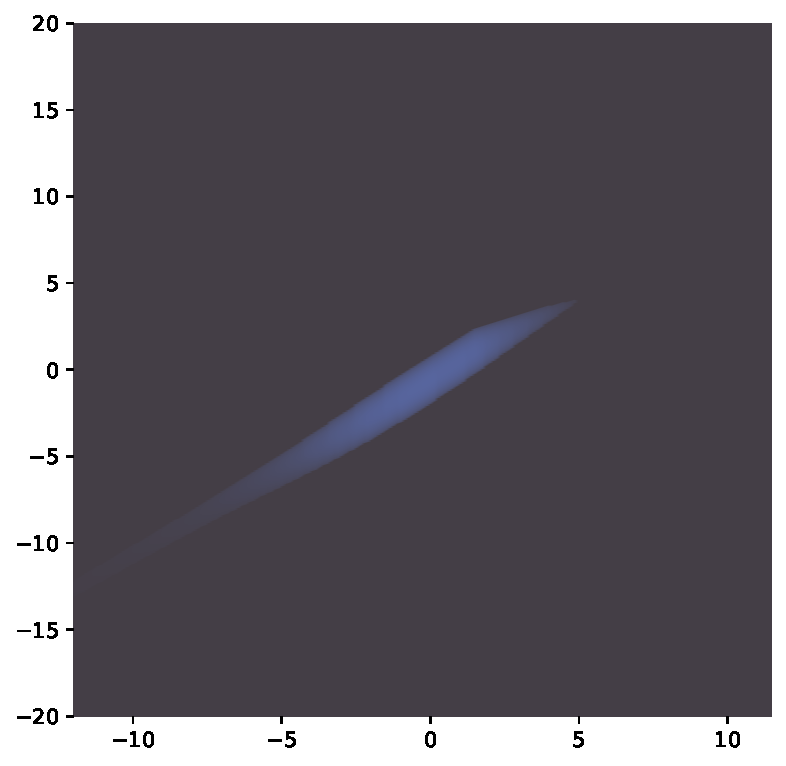
\includegraphics[height = 1.6\textwidth]{data/graph_coupure_2_30_only.pdf}};

				\end{scope}
				\begin{scope}[shift={(2,-0.3)}]
					\clip[decorate, decoration={random steps, segment length=3pt, amplitude=1pt}](8.5,-9) rectangle (13,10);
					%\draw[red]  (9,-9) rectangle (13,10);	
					\node at (0,0) [circle, ]{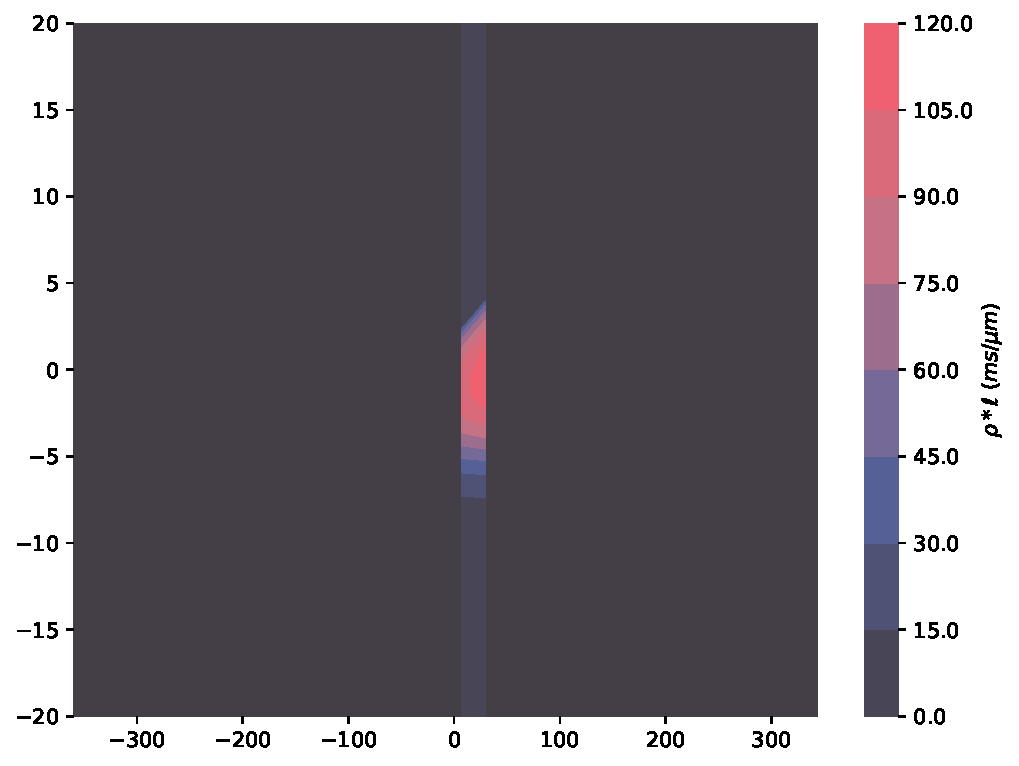
\includegraphics[height = 1.6\textwidth ]{data/complete_graph_coupure_2_0.pdf}}; 
				\end{scope}
				\node at (0,0) [circle, ] {
					\begin{tikzpicture}[transform canvas={scale=1}] 
						\Axesphase[$x/\tau ~ ( \mu m / m s )$]{$\theta ~ ( \mu m / m s ) $}
						\draw
    						(1.9, 0.2) edge[line width=1.8ex, color=\colorTwo] 
        						node[pos=1.1, below]{ \color{\colorTwo}\huge $x(s)/\tau$} (1.9, -0.2)
        					(0.2 , 1.3 ) edge[line width=1.8ex, color=\colorTwo] 
        						node[pos=1.1, left ]{ \color{\colorTwo}\huge $\theta(s)$} (-0.2 , 1.3 )
        					(1.9 , -0.2 ) edge[line width=0.8ex, color=\colorTwo , dashed ] (1.9 , 2 )
        					(-0.2 , 1.3 )  edge[line width=0.8ex, color=\colorTwo , dashed ] (3.5  , 1.3 )
        					; 
					\end{tikzpicture}};
					\draw[opacity = 0.5 , dotted , line width=0.5ex , color = \colorTwo , fill = none] 
						plot[smooth] file {data/bord_1_30.table}
						(-7,6) edge []node [pos=1.1, right ]{\huge $bord~gauche$ } ( -6.5  , 6 )	 
					;
					\draw[opacity = 0.5 , dash dot , line width=0.5ex , color = \colorTwo , fill = none] 
						plot[smooth] file {data/bord_2_30.table}
						(-7,5) edge []node [pos=1.1, right ]{\huge $bord~droite$ } ( -6.5  , 5 )	 
					;
				%\drawgrid{-10}{10}{-10}{10}
			\end{tikzpicture}
			};
	
		% density 
		\node at (0,13) [circle, ] {
			\begin{tikzpicture}[transform canvas={scale=1}] 
				\begin{scope}
					\clip[decorate, decoration={random steps, segment length=3pt, amplitude=1pt}]
        			(-9,-8) rectangle (8.5,8);
 
        			\draw[opacity = 1 , line width=1.8ex , color = \colorFour , fill = none ] plot[] file {data/density_coupure_2_30.table};
     				 \draw[line width=1.8ex , color = \colorFour] 
        				(-0.3, 5 ) edge [thick,line width=0.8ex,, color = \colorThree ]node [pos=-0.01, left  ]{\huge $107$ } ( 0.3  , 5 )	
        				(-0.3, 0 ) edge [thick,line width=0.8ex,, color = \colorThree ]node [pos=-0.01, below left ]{\huge $0$ } ( 0.3  , 0 )	
        			;


					%\drawgrid{0}{10}{0}{10}
				\end{scope}
		
				\Axesdensity[$x/\tau ~ ( \mu m / ms ) $]{$n*\tau ~( m s / \mu m )$}
				
				

        				
				%\drawgrid{-10}{10}{-10}{10}
		
			\end{tikzpicture}

			};
		
		% distribution x  
		\node at (-13,0) [circle,   rotate = 90 , xscale = 1   ] {
			\begin{tikzpicture}[transform canvas={scale=1} ] 
				\begin{scope}
					\clip[decorate, decoration={random steps, segment length=3pt, amplitude=1pt}]
        			(-9,-8) rectangle (8.5,8);

					\draw[opacity = 1 , line width=1.8ex , color = \colorFive , fill = none ] plot[smooth] file {data/Pi_coupure_2_30.table};	
					\draw[line width=1.8ex , color = \colorFour] 
    					(-0.3, 5 ) edge [thick,line width=0.8ex, color = \colorThree ]node [pos=-0.01, left  ]{\huge $107$ } ( 0.3  , 5 )	
    					(-0.3, 0 ) edge [thick,line width=0.8ex,, color = \colorThree ]node [pos=-0.01, below left ]{\huge $0$ } ( 0.3  , 0 )	
    					;			
				\end{scope}
				%\draw(1.3, 0.2) edge[line width=1.8ex, color=\colorOne] node[pos=1.1, below]{ \color{\colorOne}\huge $\theta(s)$} (1.3, -0.2);			
				\Axesdistribution[$\theta ~ ( \mu m / m s )$]{$\Pi~(m s/\mu s)  $}
				
				%\drawgrid{0}{10}{-10}{10}	
			\end{tikzpicture}

			};
	

	\end{tikzpicture}
};

%axe temporel 
\node at (0, -82) [circle ]{
	\begin{tikzpicture}[transform canvas={scale=1} ]
		\Axetemps[Expansion $\tau = 30 ~ms$]
	\end{tikzpicture}
	};


% gaduation tout 
%\drawgrid{-20}{58}{-84}{20}


\end{tikzpicture}

\end{document}
